\documentclass[11pt,preprint]{elsarticle}

\usepackage{lmodern}
%%%% My spacing
\usepackage{setspace}
\setstretch{1.2}
\DeclareMathSizes{12}{14}{10}{10}

% Wrap around which gives all figures included the [H] command, or places it "here". This can be tedious to code in Rmarkdown.
\usepackage{float}
\let\origfigure\figure
\let\endorigfigure\endfigure
\renewenvironment{figure}[1][2] {
    \expandafter\origfigure\expandafter[H]
} {
    \endorigfigure
}

\let\origtable\table
\let\endorigtable\endtable
\renewenvironment{table}[1][2] {
    \expandafter\origtable\expandafter[H]
} {
    \endorigtable
}


\usepackage{ifxetex,ifluatex}
\usepackage{fixltx2e} % provides \textsubscript
\ifnum 0\ifxetex 1\fi\ifluatex 1\fi=0 % if pdftex
  \usepackage[T1]{fontenc}
  \usepackage[utf8]{inputenc}
\else % if luatex or xelatex
  \ifxetex
    \usepackage{mathspec}
    \usepackage{xltxtra,xunicode}
  \else
    \usepackage{fontspec}
  \fi
  \defaultfontfeatures{Mapping=tex-text,Scale=MatchLowercase}
  \newcommand{\euro}{€}
\fi

\usepackage{amssymb, amsmath, amsthm, amsfonts}

\def\bibsection{\section*{References}} %%% Make "References" appear before bibliography


\usepackage[numbers]{natbib}

\usepackage{longtable}
\usepackage[margin=2.3cm,bottom=2cm,top=2.5cm, includefoot]{geometry}
\usepackage{fancyhdr}
\usepackage[bottom, hang, flushmargin]{footmisc}
\usepackage{graphicx}
\numberwithin{equation}{section}
\numberwithin{figure}{section}
\numberwithin{table}{section}
\setlength{\parindent}{0cm}
\setlength{\parskip}{1.3ex plus 0.5ex minus 0.3ex}
\usepackage{textcomp}
\renewcommand{\headrulewidth}{0.2pt}
\renewcommand{\footrulewidth}{0.3pt}

\usepackage{array}
\newcolumntype{x}[1]{>{\centering\arraybackslash\hspace{0pt}}p{#1}}

%%%%  Remove the "preprint submitted to" part. Don't worry about this either, it just looks better without it:
\makeatletter
\def\ps@pprintTitle{%
  \let\@oddhead\@empty
  \let\@evenhead\@empty
  \let\@oddfoot\@empty
  \let\@evenfoot\@oddfoot
}
\makeatother

 \def\tightlist{} % This allows for subbullets!

\usepackage{hyperref}
\hypersetup{breaklinks=true,
            bookmarks=true,
            colorlinks=true,
            citecolor=blue,
            urlcolor=blue,
            linkcolor=blue,
            pdfborder={0 0 0}}


% The following packages allow huxtable to work:
\usepackage{siunitx}
\usepackage{multirow}
\usepackage{hhline}
\usepackage{calc}
\usepackage{tabularx}
\usepackage{booktabs}
\usepackage{caption}


\newenvironment{columns}[1][]{}{}

\newenvironment{column}[1]{\begin{minipage}{#1}\ignorespaces}{%
\end{minipage}
\ifhmode\unskip\fi
\aftergroup\useignorespacesandallpars}

\def\useignorespacesandallpars#1\ignorespaces\fi{%
#1\fi\ignorespacesandallpars}

\makeatletter
\def\ignorespacesandallpars{%
  \@ifnextchar\par
    {\expandafter\ignorespacesandallpars\@gobble}%
    {}%
}
\makeatother


% definitions for citeproc citations
\NewDocumentCommand\citeproctext{}{}
\NewDocumentCommand\citeproc{mm}{%
\href{\#cite.\detokenize{#1}}{#2}\nocite{#1}}

\makeatletter
% allow citations to break across lines
\let\@cite@ofmt\@firstofone
% avoid brackets around text for \cite:
\def\@biblabel#1{}
\def\@cite#1#2{{#1\if@tempswa , #2\fi}}
\makeatother
\newlength{\cslhangindent}
\setlength{\cslhangindent}{1.5em}
\newlength{\csllabelwidth}
\setlength{\csllabelwidth}{3em}
\newenvironment{CSLReferences}[2] % #1 hanging-indent, #2 entry-spacing
{\begin{list}{}{%
	\setlength{\itemindent}{0pt}
	\setlength{\leftmargin}{0pt}
	\setlength{\parsep}{0pt}
	% turn on hanging indent if param 1 is 1
	\ifodd #1
	\setlength{\leftmargin}{\cslhangindent}
	\setlength{\itemindent}{-1\cslhangindent}
	\fi
	% set entry spacing
	\setlength{\itemsep}{#2\baselineskip}}}
{\end{list}}

\usepackage{calc}
\newcommand{\CSLBlock}[1]{\hfill\break\parbox[t]{\linewidth}{\strut\ignorespaces#1\strut}}
\newcommand{\CSLLeftMargin}[1]{\parbox[t]{\csllabelwidth}{\strut#1\strut}}
\newcommand{\CSLRightInline}[1]{\parbox[t]{\linewidth - \csllabelwidth}{\strut#1\strut}}
\newcommand{\CSLIndent}[1]{\hspace{\cslhangindent}#1}


\urlstyle{same}  % don't use monospace font for urls
\setlength{\parindent}{0pt}
\setlength{\parskip}{6pt plus 2pt minus 1pt}
\setlength{\emergencystretch}{3em}  % prevent overfull lines
\setcounter{secnumdepth}{5}

%%% Use protect on footnotes to avoid problems with footnotes in titles
\let\rmarkdownfootnote\footnote%
\def\footnote{\protect\rmarkdownfootnote}
\IfFileExists{upquote.sty}{\usepackage{upquote}}{}

%%% Include extra packages specified by user

%%% Hard setting column skips for reports - this ensures greater consistency and control over the length settings in the document.
%% page layout
%% paragraphs
\setlength{\baselineskip}{12pt plus 0pt minus 0pt}
\setlength{\parskip}{12pt plus 0pt minus 0pt}
\setlength{\parindent}{0pt plus 0pt minus 0pt}
%% floats
\setlength{\floatsep}{12pt plus 0 pt minus 0pt}
\setlength{\textfloatsep}{20pt plus 0pt minus 0pt}
\setlength{\intextsep}{14pt plus 0pt minus 0pt}
\setlength{\dbltextfloatsep}{20pt plus 0pt minus 0pt}
\setlength{\dblfloatsep}{14pt plus 0pt minus 0pt}
%% maths
\setlength{\abovedisplayskip}{12pt plus 0pt minus 0pt}
\setlength{\belowdisplayskip}{12pt plus 0pt minus 0pt}
%% lists
\setlength{\topsep}{10pt plus 0pt minus 0pt}
\setlength{\partopsep}{3pt plus 0pt minus 0pt}
\setlength{\itemsep}{5pt plus 0pt minus 0pt}
\setlength{\labelsep}{8mm plus 0mm minus 0mm}
\setlength{\parsep}{\the\parskip}
\setlength{\listparindent}{\the\parindent}
%% verbatim
\setlength{\fboxsep}{5pt plus 0pt minus 0pt}



\begin{document}



\begin{frontmatter}  %

\title{Report Loans and credit}

% Set to FALSE if wanting to remove title (for submission)




\author[Add1]{Tatjana Ebert}
\ead{}








\vspace{1cm}





\vspace{0.5cm}

\end{frontmatter}

\setcounter{footnote}{0}



%________________________
% Header and Footers
%%%%%%%%%%%%%%%%%%%%%%%%%%%%%%%%%
\pagestyle{fancy}
\chead{}
\rhead{}
\lfoot{}
\rfoot{\footnotesize Page \thepage}
\lhead{}
%\rfoot{\footnotesize Page \thepage } % "e.g. Page 2"
\cfoot{}

%\setlength\headheight{30pt}
%%%%%%%%%%%%%%%%%%%%%%%%%%%%%%%%%
%________________________

\headsep 35pt % So that header does not go over title




\section{Netflix Content Strategy
Analysis}\label{netflix-content-strategy-analysis}

\subsection{Introduction}\label{introduction}

Netflix has recently faced pressure from declining subscriber growth and
a sharp fall in its share price. In this context, understanding what
types of content perform well on streaming platforms is important for
investors considering the launch of a competing service.

This report uses the Netflix IMDb title data provided up to 2023, with
the movie analysis restricted to titles released up to 2022. The focus
is on identifying patterns in movie origin, genre, IMDb ratings,
runtime, and textual descriptions. Where useful, HBO data is used as a
benchmark to compare content strategy across platforms.

\subsection{Data and Methodology}\label{data-and-methodology}

The analysis uses the Netflix titles, credits and movie information
datasets supplied for the question. The data contains information on
title type, production country, genre, IMDb rating, runtime, description
and credits. The analysis focuses on movies, as requested in the brief.

The following methods are used:

\begin{itemize}
\tightlist
\item
  Frequency analysis to identify dominant countries and genres.
\item
  Boxplots and summary tables to compare IMDb ratings and runtime by
  country.
\item
  Textual analysis of descriptions using word frequencies and TF-IDF to
  identify distinctive country-specific themes.
\item
  Platform comparison using HBO data where relevant.
\end{itemize}

\subsection{Country Representation}\label{country-representation}

\begin{figure}[H]

{\centering 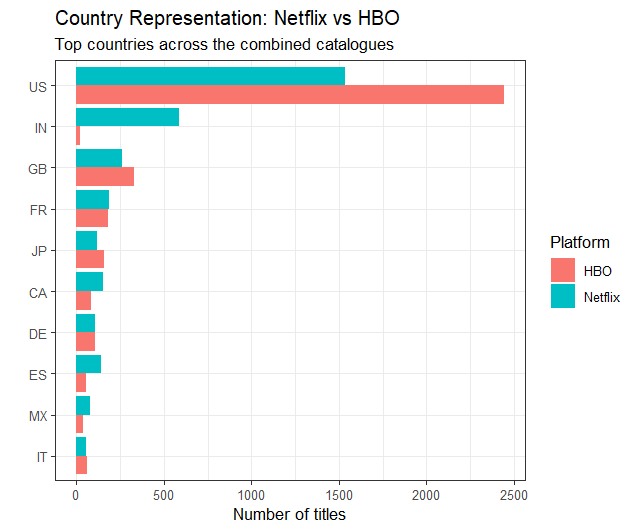
\includegraphics[width=0.9\linewidth]{../../graphs/country_rep} 

}

\caption{Country representation of Netflix movies. \label{fig:country_rep}}\label{fig:country_rep}
\end{figure}

Figure \ref{fig:country_rep} shows that Netflix's movie catalogue is
heavily concentrated in a small number of production markets. The United
States is the dominant contributor, followed by other large
film-producing countries such as India and the United Kingdom.

This suggests that Netflix relies strongly on countries with established
film industries and large domestic audiences. For a new streaming
platform, this implies that catalogue scale is likely to depend on
securing content from major global production hubs rather than
attempting to build all content internally.

\begin{figure}[H]

{\centering 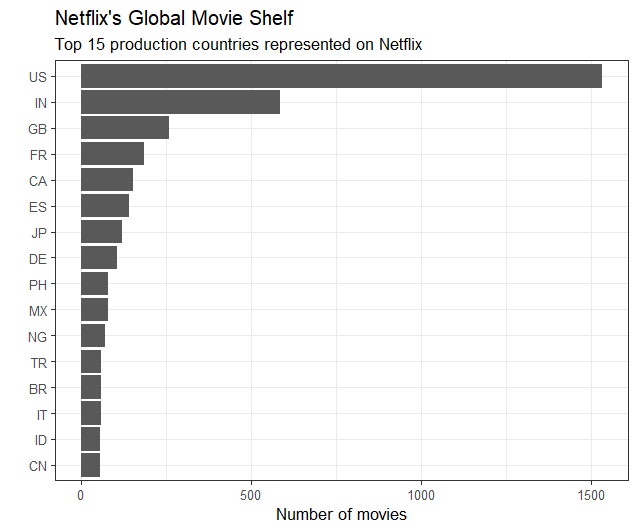
\includegraphics[width=0.9\linewidth]{../../graphs/countries} 

}

\caption{Top countries by number of Netflix movies. \label{fig:countries}}\label{fig:countries}
\end{figure}

Figure \ref{fig:countries} confirms that Netflix's content supply is not
evenly distributed across countries. A few countries account for a large
share of available movies, while many other countries are represented by
far fewer titles.

\subsection{IMDb Ratings by Country}\label{imdb-ratings-by-country}

\begin{figure}[H]

{\centering 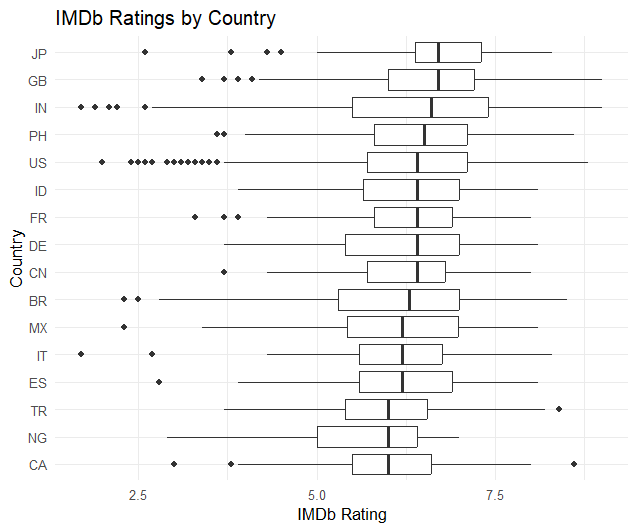
\includegraphics[width=0.9\linewidth]{../../graphs/Rating_by_country} 

}

\caption{IMDb rating distribution by production country. \label{fig:rating_country}}\label{fig:rating_country}
\end{figure}

Figure \ref{fig:rating_country} compares IMDb ratings across the major
production countries. The results show that countries with the largest
number of titles do not necessarily have the highest median ratings.
This is important because it indicates that catalogue size and content
quality are not the same strategic objective.

For investors, the implication is that a streaming service should not
only compete on volume. Smaller but higher-quality international
catalogues may provide stronger audience satisfaction and
differentiation.

\subsection{Runtime Analysis}\label{runtime-analysis}

\begin{figure}[H]

{\centering 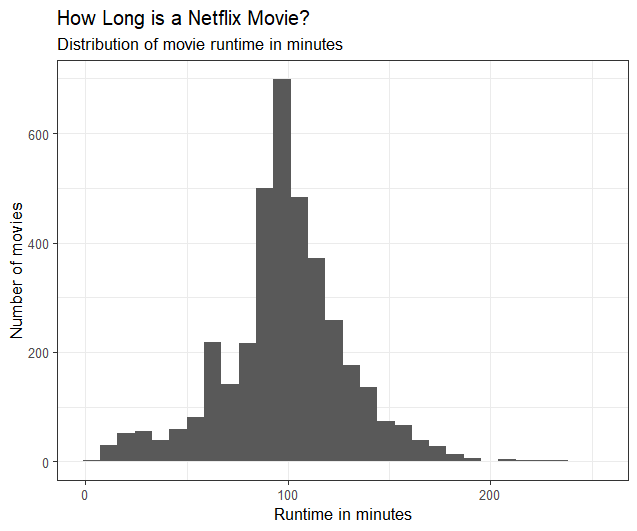
\includegraphics[width=0.9\linewidth]{../../graphs/runtime} 

}

\caption{Distribution of Netflix movie runtime. \label{fig:runtime}}\label{fig:runtime}
\end{figure}

Figure \ref{fig:runtime} shows that Netflix movies are mostly
concentrated around the standard feature-film length of roughly 90 to
120 minutes. This suggests that, despite the flexibility of streaming
platforms, movie runtimes still follow traditional viewing preferences.

\begin{figure}[H]

{\centering 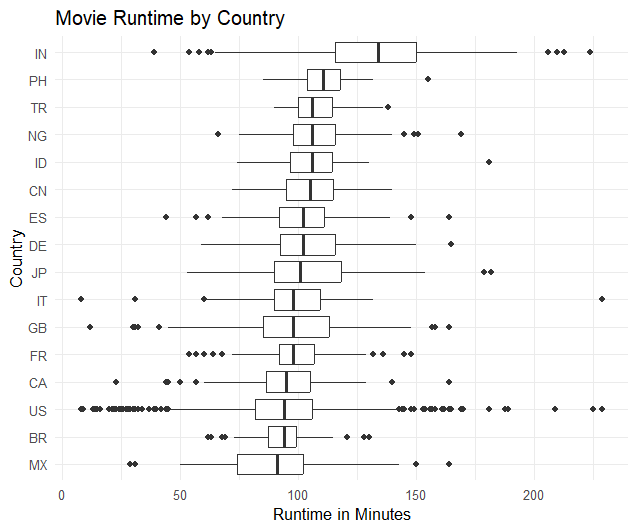
\includegraphics[width=0.9\linewidth]{../../graphs/runtime_by_countries} 

}

\caption{Netflix movie runtime by country. \label{fig:runtime_country}}\label{fig:runtime_country}
\end{figure}

Figure \ref{fig:runtime_country} shows that runtime differs by
production country. These differences may reflect local storytelling
traditions, audience expectations and industry norms.

\begin{figure}[H]

{\centering 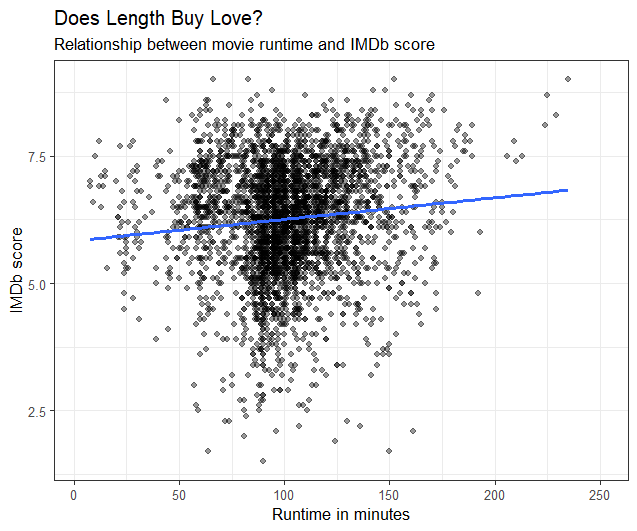
\includegraphics[width=0.9\linewidth]{../../graphs/Correlation_Runtime_Rating} 

}

\caption{Relationship between runtime and IMDb rating. \label{fig:corr_runtime_rating}}\label{fig:corr_runtime_rating}
\end{figure}

Figure \ref{fig:corr_runtime_rating} indicates that the relationship
between runtime and IMDb rating is weak. Longer movies are not
automatically better rated. From a strategic perspective, this suggests
that investing in longer productions does not necessarily improve
audience reception.

\subsection{Genre Analysis}\label{genre-analysis}

\begin{figure}[H]

{\centering 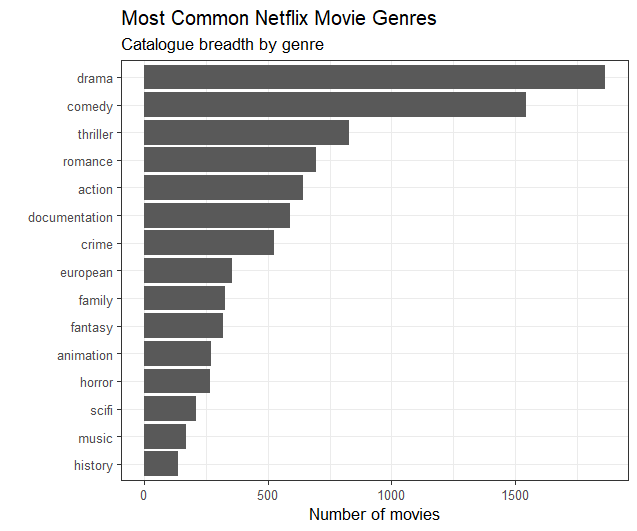
\includegraphics[width=0.9\linewidth]{../../graphs/genres} 

}

\caption{Most common Netflix movie genres. \label{fig:genres}}\label{fig:genres}
\end{figure}

Figure \ref{fig:genres} shows that Netflix's movie catalogue is
dominated by broad mainstream genres such as drama, comedy and action.
These genres are likely used because they appeal to wide audiences and
are suitable for global distribution.

\begin{figure}[H]

{\centering 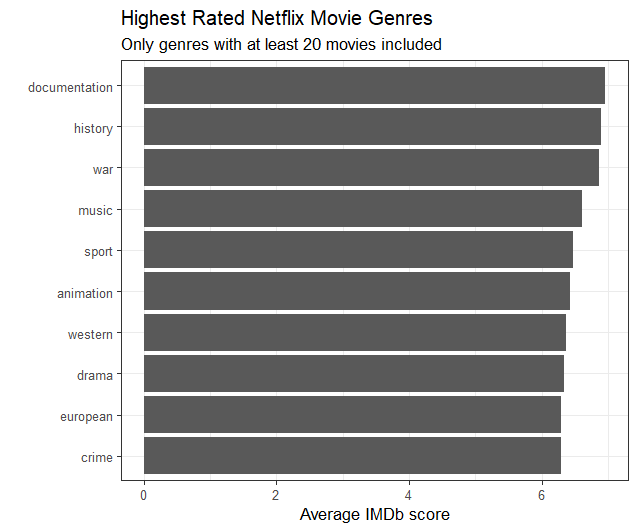
\includegraphics[width=0.9\linewidth]{../../graphs/Genres_high} 

}

\caption{Highest-rated Netflix movie genres. \label{fig:genres_high}}\label{fig:genres_high}
\end{figure}

Figure \ref{fig:genres_high} shows that the most common genres are not
always the highest rated. This suggests that niche or less frequent
genres may offer stronger audience satisfaction. A new streaming
platform may therefore benefit from targeted investment in high-quality
niche genres rather than simply copying Netflix's high-volume genre
strategy.

\subsection{Textual Analysis of Movie
Descriptions}\label{textual-analysis-of-movie-descriptions}

\begin{figure}[H]

{\centering 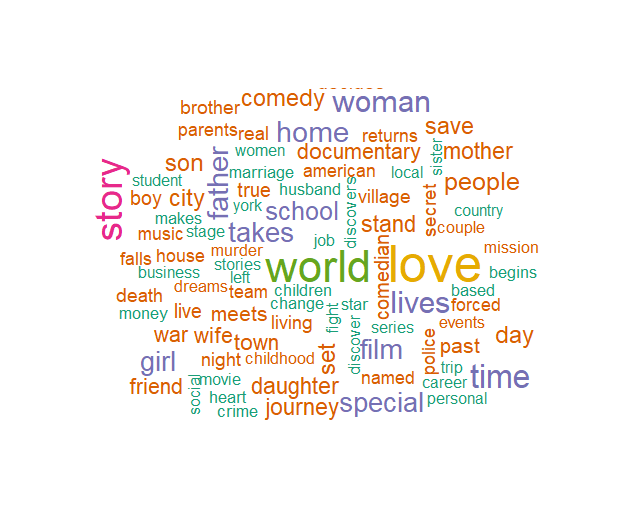
\includegraphics[width=0.8\linewidth]{../../graphs/wordcloud} 

}

\caption{Most common words in Netflix movie descriptions. \label{fig:wordcloud}}\label{fig:wordcloud}
\end{figure}

Figure \ref{fig:wordcloud} summarises the most frequent words in Netflix
movie descriptions. The dominant words suggest that Netflix movies often
focus on broad and relatable themes such as family, love, life,
relationships, crime and personal conflict.

\begin{figure}[H]

{\centering 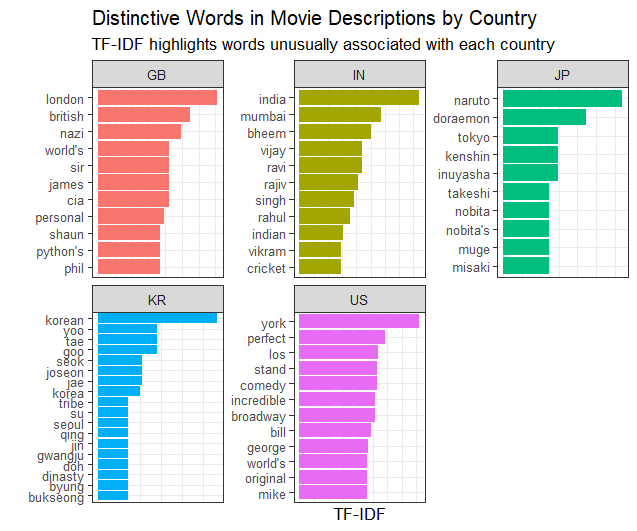
\includegraphics[width=0.95\linewidth]{../../graphs/words_by_country} 

}

\caption{Distinctive words in movie descriptions by country. \label{fig:words_country}}\label{fig:words_country}
\end{figure}

Figure \ref{fig:words_country} provides a more informative
country-specific view using TF-IDF. This shows which words are
especially distinctive for selected countries. The results indicate that
countries differ not only in the number of movies they produce, but also
in the type of stories they contribute.

This is particularly relevant for the task, since it shows that movie
preferences and themes vary across countries. A successful streaming
strategy should therefore consider regional storytelling preferences
instead of relying on a single global content formula.

\subsection{Director Analysis}\label{director-analysis}

\begin{figure}[H]

{\centering 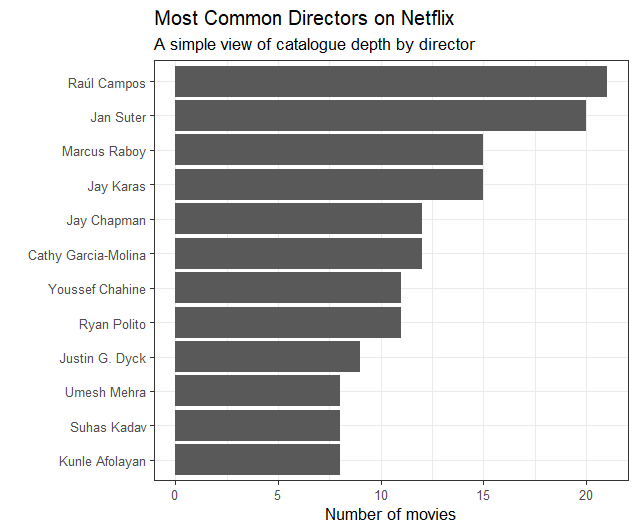
\includegraphics[width=0.9\linewidth]{../../graphs/directors} 

}

\caption{Most common directors represented in the Netflix movie catalogue. \label{fig:directors}}\label{fig:directors}
\end{figure}

Figure \ref{fig:directors} shows the directors most frequently
represented in the Netflix movie catalogue. While this is less central
than country, genre and rating analysis, it provides evidence of
Netflix's reliance on repeat contributors. This may reflect long-term
production relationships or the acquisition of multiple films from the
same creators.

\subsection{Netflix and HBO
Comparison}\label{netflix-and-hbo-comparison}

\begin{figure}[H]

{\centering 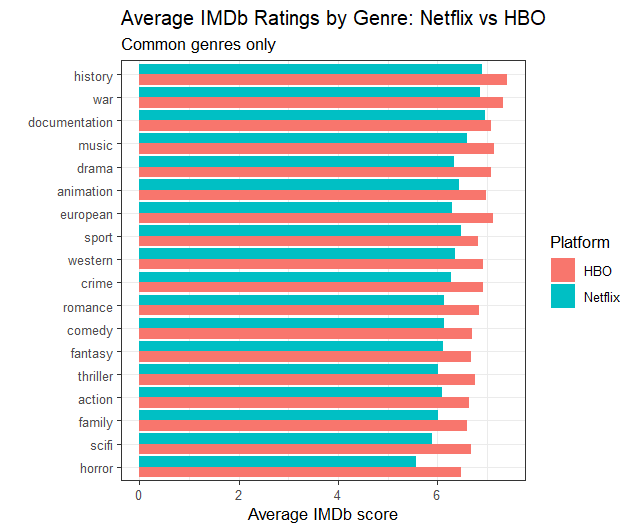
\includegraphics[width=0.9\linewidth]{../../graphs/HBO_genre} 

}

\caption{Average IMDb ratings by genre: Netflix versus HBO. \label{fig:hbo_genre}}\label{fig:hbo_genre}
\end{figure}

Figure \ref{fig:hbo_genre} compares average IMDb ratings by genre
between Netflix and HBO. The comparison highlights differences in
platform strategy. Netflix appears to focus more on catalogue breadth,
while HBO is often associated with a more selective and
prestige-oriented catalogue.

\begin{figure}[H]

{\centering 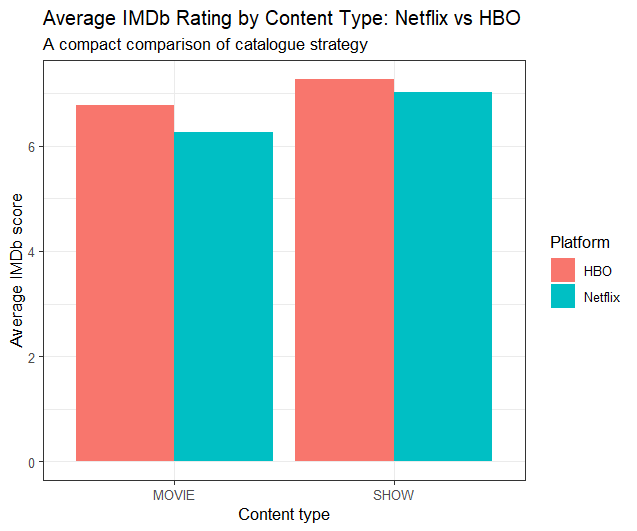
\includegraphics[width=0.9\linewidth]{../../graphs/HBO_rating} 

}

\caption{Average IMDb rating comparison between Netflix and HBO. \label{fig:hbo_rating}}\label{fig:hbo_rating}
\end{figure}

Figure \ref{fig:hbo_rating} reinforces this difference. If HBO achieves
higher average ratings in certain categories, this suggests that a
smaller but more carefully curated catalogue can compete against a
larger content library.

\subsection{Strategic Implications}\label{strategic-implications}

The analysis provides several useful insights for investors considering
a new streaming service.

First, Netflix's catalogue is strongly concentrated in major production
countries. This means that market entry would likely require
partnerships with established content-producing regions.

Second, high catalogue volume does not guarantee high IMDb ratings. A
new platform should therefore avoid competing only on quantity and
should instead identify high-performing regions and genres.

Third, runtime is not strongly related to rating. This suggests that
content quality, genre and story appeal matter more than movie length.

Fourth, textual analysis shows that movie themes differ across
countries. Regional content strategies may therefore be important for
international growth.

Finally, the HBO comparison suggests that a smaller, more curated
catalogue may be a viable alternative to Netflix's scale-based model.

\subsection{Conclusion}\label{conclusion}

The Netflix data suggests that successful streaming content strategy
depends on more than catalogue size. The strongest investment case lies
in balancing international diversity, high-quality genres, regional
storytelling preferences and careful content curation.

For a new streaming service, the key lesson is not to replicate
Netflix's scale immediately. Instead, investors should consider a
focused strategy built around high-rated genres, distinctive
international content and regionally relevant themes.

\begin{verbatim}
\end{verbatim}

\newpage

\bibliography{Tex/ref}





\end{document}
